\documentclass[conference]{IEEEtran}

\usepackage{graphicx}  
\usepackage[margin=2.5cm]{geometry}
\usepackage{breakcites}
\usepackage{indentfirst}
\usepackage{pgfgantt}
\usepackage{pdflscape}
\usepackage{float}
\usepackage{epsfig}
\usepackage{epstopdf}
\usepackage[cmex10]{amsmath}
\usepackage{stfloats}
\usepackage{multirow}
\usepackage{multicol}


\renewcommand{\refname}{REFERENCES}
\linespread{1.3}

\usepackage{mathtools}
%\newcommand{\HRule}{\rule{\linewidth}{0.5mm}}
\thispagestyle{empty}
\begin{document}


\title{BLG 202E \\Numerical Methods \\ \\SVD-Based Digital Image Watermarking Scheme}

\author{\IEEEauthorblockN{Ali Emre Kaya \\150210097}
\IEEEauthorblockA{\textit{Computer Engineering Department} \\
\textit{Istanbul Technical University}\\
Spring 2024}
}

\maketitle




\thispagestyle{empty}
\addtocontents{toc}{\contentsline {section}{\numberline {}FRONT COVER}{}}
\addtocontents{toc}{\contentsline {section}{\numberline {}CONTENTS}{}}
\setcounter{tocdepth}{4}
\tableofcontents


\setcounter{page}{1}
\vspace{30pt}

\begin{abstract}
Watermarking is the process of embedding information into digital media for various purposes such as copyright protection and content authentication. This paper presents an implementation of an SVD-based digital image watermarking scheme proposed by Chang et al.
\end{abstract}

\section{Problem}
Watermarking is the process of embedding information (the watermark) into digital media such as images, audio, video, or documents. Watermarking serves various purposes, including copyright protection, content authentication, ownership verification, and content tracking. In this way, it can be identified who owns the original picture even after operations such as duplication or modification.

SVD (Singular Value Decomposition) based watermarking is a technique that utilizes the mathematical properties of SVD to embed watermarks into digital media. SVD decomposes a matrix into three matrices: $U$, $\Sigma$, and $V^T$. In the context of watermarking, the original media content is represented as a matrix, and the watermark is embedded by modifying the singular values or vectors of the SVD decomposition.

In this project, I will reimplement the SVD-based digital watermarking scheme proposed by Chang et al.

\section{Implementation Details}
\subsection{SVD Implementation}
In the SVD implementation, I utilized the power method for initialization. This method facilitated the decomposition of the image matrix into its constituent components: the left singular vectors (U), the singular values ($\Sigma$), and the right singular vectors ($V^T$). If we want to find all the eigenvalues and vectors, we should eliminate the dominant direction from the matrix, and the most dominant singular value should be found again. In order to accomplish that, we might use singular values and previously computed left and right singular vectors to subtract the prior eigenvector(s) component(s) from the original matrix. By employing the power method as I mentioned before, I enable the efficient extraction of the essential components of the image representation.
\subsection{Watermark Embedding Procedure}
To embed a watermark in the host image, I use Chang and colleagues' procedure. Firstly, I partition the host image into blocks for each watermark bit, and I use the proper algorithm for embedding. After embedding all the bits, I reconstruct all the blocks to obtain a watermarked image.
\subsection{Watermark Extracting Procedure}
For the extraction of watermark from the host image, I use Chang and colleagues' algorithm. It is like the embedding procedure's reverse order, but the algorithm is different. I partitioned the watermarked image into blocks for extracting bits. Then I store these bits, and while all the blocks's embedding watermark bits are extracted, I convert them into an image that I foresee resembling the watermark image.

\section{Dataset}
\subsection{Watermark Image}
I chose IEEE's logo as a watermark image. I arrange it's size at $32x32$. Also, the watermark should only consist of two different bits, 0 (black) and 1 (white). To achive that; firstly I convert it to gray scale, then I determine a treshold value, if bit's value is less that treshold value, bit will be 0, otherwise bit will be 1.
\subsection{Host Image}
I chose a llama picture as a host image. I arrange it to be a multiple of 2. I also convert it to the gray scale. After that, I adjusted this image to be the largest square it could be.

\vspace{30pt}
\section{Experiments}

In the first part of the project, I added my host and watermarked image.

\begin{figure}[h]
    \centering
    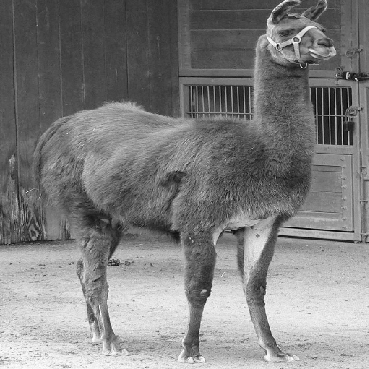
\includegraphics[width=0.5\textwidth, angle=0]{images/output_host_image.png}
    \caption{Original host image}
    \label{fig1}
\end{figure}


\begin{figure}[h]
    \centering
    
\includegraphics[width=0.2\textwidth, angle=0]{images/output_watermark.png}
    \caption{Watermark}
    \label{fig2}
\end{figure}

After that, I used the implemented embed and extract method to embed watermark in the host image, and after that, I extracted watermark from the watermarked image. I measured the image quality with the peak signal-to-noise ratio ($PSNR$) among the watermarked and original host images, and the rate I got was 53 dB. That means embedding procedures cause little distortion on images, so differences between two images are not understandable by human eyes.
\newpage
\begin{figure}[h]
    \centering
    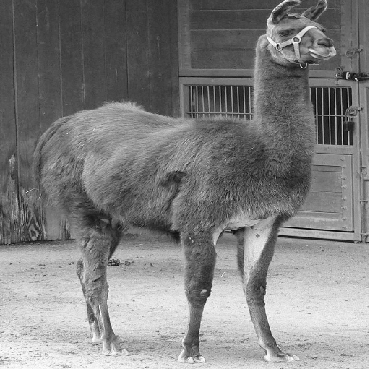
\includegraphics[width=0.5\textwidth, angle=0]{images/output_watermarked_image.png}
    \caption{Watermarked image}
    \label{fig3}
\end{figure}

\begin{figure}[h]
    \centering
    
\includegraphics[width=0.2\textwidth, angle=0]{images/output_watermark_extracted.png}
    \caption{Extracted watermark from watermarked image}
    \label{fig4}
\end{figure}

Finally, I extracted the watermark from a tampered image and checked whether the watermark was still understandable.
\newpage

\begin{figure}[h]
    \centering
    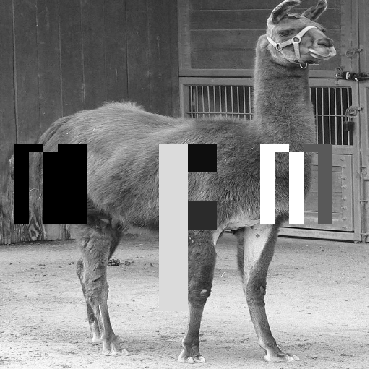
\includegraphics[width=0.5\textwidth, angle=0]{images/output_tampered_image.png}
    \caption{Tampered image}
    \label{fig5}
\end{figure}

\begin{figure}[h]
    \centering
    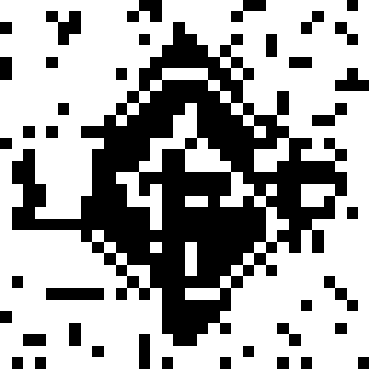
\includegraphics[width=0.2\textwidth, angle=0]{images/output_watermark_extracted_fromTampered.png}
    \caption{Extracted watermark from tampered image}
    \label{fig6}
\end{figure}

As can be seen in Fig 6, the IEEE logo is distinguishable, although not as easily as that extracted from the watermarked image.





\bibliographystyle{unsrt}
\bibliography{reference}
\cite{CHANG20051577}
\cite{hinno2021simple}



\end{document}

